\documentclass[talk.tex]{subfiles}
\begin{document}


    	\begin{tikzpicture}[scale=.7]
    		\newcommand{\orig}{-1.5}
    		\newcommand{\trans}{1.5}
    		\newcommand{\vertspac}{-2.}
    		\newcommand{\vertsize}{0} % vertical spand of the rectangles
    		\newcommand{\del}{.2}
    		\newcommand{\rad}{2pt} % radii of the circles
    	
    		% set the style of the strong bonds
    		\tikzset{
    			strong/.style={
    				double,
    				double distance=\rad,
    				line width=0.5pt
    				}
    		}
    		
    		% initial chain
    	
    		% bonds 
        	\draw[-] (\orig, 0)  node [left] {}  -- (\orig+\trans, 0)  node [midway, above] {$t_w$};
			\draw[strong] (\orig+\trans,0) -- (\orig+2*\trans,0)  node [midway, above] {$t_s$};
			\draw[-] (\orig+2*\trans,0) -- (\orig+3*\trans,0) node [midway, above] {$t_w$};	
			\draw[strong] (\orig+3*\trans,0) -- (\orig+4*\trans,0) node [midway, above] {$t_s$};
			\draw[-] (\orig+4*\trans,0) -- (\orig+5*\trans,0) node [midway, above] {$t_w$};
			\draw[-] (\orig+5*\trans,0) -- (\orig+6*\trans,0) node [midway, above] {$t_w$};
			\draw[strong] (\orig+6*\trans,0) -- (\orig+7*\trans,0) node [midway, above] {$t_s$};
			\draw[-] (\orig+7*\trans,0) -- (\orig+8*\trans,0) node [midway, above] {$t_w$};
    	
    		% sites
			\foreach \x in {0,...,7}
		      \filldraw (\orig+\x*\trans,0) circle (\rad); % node [below] {$\ket{\x}$};
		    % last site with chain step attached
		    \filldraw (\orig+8*\trans,0) circle (\rad) node [right] {~~~$n$};
		    
		    % rectangles around atoms
%		    \draw [rounded corners] (\orig-\vertsize,-\vertsize) rectangle (\orig+\vertsize,\vertsize);
%		    \draw [rounded corners] (\orig-\vertsize+5*\trans,-\vertsize) rectangle (\orig+\vertsize+5*\trans,\vertsize);
%		    \draw [rounded corners] (\orig-\vertsize+8*\trans,-\vertsize) rectangle (\orig+\vertsize+8*\trans,\vertsize);
		    
		    % arrows below rectangles
		    \draw [->] (\orig,-\vertsize-\del) -- (\orig,\vertspac+\del);
		    \draw [->] (\orig+5*\trans,-\vertsize-\del) -- (\orig+5*\trans,\vertspac+\del);
		    \draw [->] (\orig+8*\trans,-\vertsize-\del) -- (\orig+8*\trans,\vertspac+\del);
		      
		    % atomic chain
		    
        	\draw[-] (\orig, \vertspac)  node [left] {}  -- (\orig+5*\trans, \vertspac)  node [midway, above] {\only<1>{$t_w'$} \only<2>{$\zb t_w$}};
			\draw[strong] (\orig+5*\trans,\vertspac) -- (\orig+8*\trans,\vertspac) node [midway, above] {\only<1>{$t_s'$} \only<2>{$\zb t_s$}};
			
			\filldraw (\orig,\vertspac) circle (\rad); % node [below] {$\ket{\x}$};
			\filldraw (\orig+5*\trans,\vertspac) circle (\rad); % node [below] {$\ket{\x}$};
			\filldraw (\orig+8*\trans,\vertspac) circle (\rad) node [right] {~~~$n-3$};
		\end{tikzpicture}

\end{document}